\chapter{Implemenations and Evaluations}

This chapter presents details of the implementations, experiments and evaluations for the proposed models in previous chapter. Section \ref{sec:chap4_implementation} describes the architecture of training system written in Torch framework which was used to train all the models. Before going onto detailed experiments and evaluations, section \ref{sec:chap4_metric} provides explanation for the metrics used to evaluate models' performances includeng BLUE, METEOR and CIDEr scores. Subsequently, section \ref{sec:chap4_experiment} presents all the experiments along with evaluation and assessment for each of them.

%% -------------------------------------
%% SECTION 1:
%%   Implementations
%% -------------------------------------
\section{Implementations}
\label{sec:chap4_implementation}


\subsection{Training System Architecture}

\subsection{Training and Monitoring}
Training a deep neural network can be very hard and time-consuming. During the course of training of all models and experiments presented in this thesis, I have followed several guidelines \cite{bottou-tricks-2012} on tips and tricks to effectively train deep neural networks.
	
	\subsubsection{Choosing a right learning rate}
	As shown in \cite{Murata98astatistical}, the mathematics of stochastic gradient descent do not depend on the size of training set. Therefore, the best way to determine the correct learning rates is to perform experiments on a small but representative traing set. When the model performs well on training cost with the sample training set with some learning rate $\gamma_t$, we can apply that learning rate to train our model on real training set.

	For this purpose, I set up a small experiment on subset of MSCOCO dataset (see \ref{sec:dataset_mscoco} for details). The subset COCO-1k consists of images randomly from MSCOCO training set. There are in total $1,200$ images in COCO-1k; $1,000$ of them are in training set and the rest are reserved in the validation set. I trained a model with 16-layer VGGNet as CNN; optimization method is SGD; the LSTM has 512 hidden units and with batch size equals to 5.

	\subsubsection{Monitoring the training process}
	\label{sec:monitoring}

%% -------------------------------------
%% SECTION 3:
%%   Experimental Environment
%% -------------------------------------
\section{Experimental Environment}
\label{sec:chap4_environment}

\subsection{Hardware configurations}
\label{sec:hardware}
All models are trained with the hardware configurations as shown in table \ref{tab:hardware_configuration}. Though the $GK210B$ board has two Tesla K80s, all the experiments were conducted in a single GPU for the sake of simplicity.

\begin{table}
	\centering
	\caption{Hardware configuration for training all models}	
	\label{tab:hardware_configuration}
	\begin{tabularx}{0.65\textwidth}{ll}
		\toprule
		CPU & 2 x Intel(R) Xeon(R) E5-2620v3 \\
			& (6 cores, 15MB cache, 2.40GHz) \\
		\midrule
		Memory & 4 x 32 GB ECC Registered \\
		\midrule 
		GPU & 2 x nVidia Tesla K80 [GK210B], \\
			& each with $2,496$ CUDA cores, \\
			& $12$GB VRAM, 240 GB/s memory bandwidth \\
		\midrule
		Storage & 8 x 6TB SATA 7200RPM Enterprise \\
		\bottomrule
	\end{tabularx}
\end{table}

\subsection{Datasets}
\subsubsection{Flickr8k}
Flickr8K was first proposed by \cite{Hodosh:2013:FID:2566972.2566993} as a benchmark collection for sentence-based image description and search. The dataset consists of $8,000$ images accompanied with five different description sentences which provide clear description of salient entities and events. \textit{TODO: re-paraphrase}
\subsubsection{Flickr30k}
As introduced in \cite{DBLP:journals/tacl/YoungLHH14}, Flickr30k is an extension of Flickr8k. The dataset is comprised of $158,915$ crowd-sourced captions describing $31,783$ images. Except for images that overlapped in Flickr8k, the new images and captions in this dataset focus on people involved in everyday activities and events.

Several examples of images and captions in Flickr8K and Flickr30k are shown in figure \ref{fig:flickr-examples}.

\begin{figure}
	\centering
	\begin{tabular}{l l}
		\toprule
		\multirow{5}{*}{\includegraphics[width=0.25\linewidth]{Chapters/Fig/black_dog_running_fence.jpg}} & \parbox{11cm}{\small{A black and white dog is running in a grassy garden surrounded by a white fence}} \\
		& \small{A black and white dog is running through the grass} \\
		& \small{A Boston terrier is running in the grass} \\
		& \small{A Boston Terrier is running on lush green grass in front of a white fence} \\
		& \small{A dog runs on the green grass near a wooden fence} \\
		\midrule
		\begin{minipage}{0.25\linewidth}
			\centering
			\includegraphics[width=0.8\linewidth]{Chapters/Fig/men_red_helmet_riding_bike_rocks.jpg}
		\end{minipage}
		&
		\begin{minipage}{0.75\linewidth}
			\parbox{11cm}{\small{A boy in a black helmet and red long sleeve shirt rides his motorbike over a rocky stream}} \\
			\small{A man on a motorcycle steers through swampy terrain} \\
			\small{A man rides his bike over rocks and a creek.} \\
			\small{A motocross bike is being ridden between markers in a running stream.} \\
			\small{A person is dirt biking over rocks and water.}
		\end{minipage}\\
		\midrule
		\begin{minipage}{0.25\linewidth}
			\includegraphics[width=\linewidth]{Chapters/Fig/flickr/9950913.jpg}
		\end{minipage}
		&
		\begin{minipage}{0.75\linewidth}
			\parbox{11cm}{\small{A group of people are wearing signs that say on strike while someone is speaking at a booth with the Presidential seal.}} \\
			\small{A strike is currently going on and there are lots of people.} \\
			\small{A person speaks at a protest on a college campus.} \\
			\small{A woman is speaking at a podium outdoors.} \\
			\small{Members of a strike at Yale University.}
		\end{minipage}\\
		\midrule
		\begin{minipage}{0.25\linewidth}
			\centering
			\includegraphics[width=0.7\linewidth]{Chapters/Fig/flickr/23016250.jpg}
		\end{minipage}
		&
		\begin{minipage}{0.5\linewidth}
			\parbox{11cm}{\small{A young woman plays tennis while wearing a yellow outfit.}} \\
			\small{A woman wearing a yellow outfit is holding a racket.} \\
			\small{A woman tennis player reacts after hitting the ball.} \\
			\small{There is a woman in yellow playing tennis.} \\
			\small{Woman in yellow playing tennis.}
		\end{minipage}\\
		
		\midrule
		\begin{minipage}{0.25\linewidth}
			\centering
			\includegraphics[width=\linewidth]{Chapters/Fig/flickr/46360594.jpg}
		\end{minipage}
		&
		\begin{minipage}{0.6\linewidth}
			\parbox{11cm}{\small{Two girls are seated behind a table festooned with toys, including a blue Furby, two pink bunny dolls, and assorted figurines and stuffed animals.}} \\
			\small{Two young girls are positioned behind a table covered in various toys and miniatures.} \\
			\small{Two kids sitting at a table full of toys.} \\
			\small{Two young girls selling trinkets.} \\
			\small{Two young girls selling toys.}
		\end{minipage}\\
		
		\midrule
		\begin{minipage}{0.25\linewidth}
			\centering
			\includegraphics[width=0.8\linewidth]{Chapters/Fig/flickr/141126420.jpg}
		\end{minipage}
		&
		\begin{minipage}{0.6\linewidth}
			\parbox{11cm}{\small{Guy in black wetsuit is riding a wave with a white surfboard.}} \\
			\small{A man is surfing in a wetsuit and is coming out of the curl.} \\
			\small{A man in a wetsuit catches a wave on his white surfboard.} \\
			\small{A man in a black wetsuit surfs on a whiteboard.} \\
			\small{A man in a black wetsuit is surfing on a wave.}
		\end{minipage}\\
		
		\midrule
		\begin{minipage}{0.25\linewidth}
			\centering
			\includegraphics[width=\linewidth]{Chapters/Fig/flickr/166654939.jpg}
		\end{minipage}
		&
		\begin{minipage}{0.5\linewidth}
			\parbox{11cm}{\small{Race cars are racing each other on a dirt racetrack and the green one is in the lead.}} \\
			\small{Two lines of colorful cars racing on a racetrack.} \\
			\small{Ralley cars muscle for position on a dirt track.} \\
			\small{A group of race buggies travel down a racetrack.} \\
			\small{Cars racing on a dirt track.}
		\end{minipage}\\
		\bottomrule
	\end{tabular}
	\caption[Sample images in Flickr8k and Flickr30k]{Sample images in Flickr8k and Flickr30k. Each comes with 5 crow-sourced captions. Images in those dataset vary significantly in terms of object classes, activities, themes, etc.}
	\label{fig:flickr-examples}
	
\end{figure}

\subsubsection{MSCOCO}
\label{sec:dataset_mscoco}

MSCOCO \cite{DBLP:journals/corr/LinMBHPRDZ14} (Microsoft Common Objects in Context) is a large-scale dataset that addresses three core research problems in scene understanding: detecting non-iconic views of objects, contextual reasoning between objects and the precise 2D localization of objects. It has been considered as the start-of-the-art dataset for numerous computer vision tasks (e.g., image classification, object detection, object segmentation, scene labelling, etc.). The dataset has approximately $328,000$ images of complex everyday scenes containing common objects in their natural context. Like in aforementioned Flickr8k \& Flickr30k datasets, each images in MSCOCO is also associated with five caption sentences that describe the content of such image.

The statistics of the datasets are summarized in table \ref{tab:dataset-statistics}
\begin{table}
	\centering
	\label{tab:dataset-statistics}
	\begin{tabular}{lccc}
		\toprule
		\multirow{2}{*}{Dataset name} & \multicolumn{3}{c}{size} \\ \cline{2-4}
		& train & validation & test \\ \midrule
		Flickr8k & 6000 & 1000 & 1000 \\
		Flickr30K & 28000 & 1000 & 1000 \\
		MSCOCO & 82783 & 40504 & 40775 \\
		\bottomrule
	\end{tabular}
	\caption{Dataset statistics}
\end{table}


%% -------------------------------------
%% SECTION 4:
%%   Experiments
%% -------------------------------------
\section{Experiments and Evaluations}
\label{sec:chap4_experiment}

This section gives the details of all experiments that we have conducted to explore and evaluate different models as well as the effects of different hyperparameters to the models proposed in previous chapter. To ensure the objectivity, when comparing a certain hyperparameter, all the other ones are fixed within an experiment. 

The organization of this section is as follow. In section \ref{exp:optim}, we perform experiments to select appropriate optimization algorithm for our models by two criterion: convergent speed and best achieved performance. Next, section \ref{exp:lstm_architecture} suggests a optimal LSTM decoder as a trade-off between performance and deployability of our models. Section \ref{exp:cnn} compares the effects different visual feature extractors \gls{cnn} to the performance of our models. Finally, section \ref{exp:transfer_learning} studies the transfer learning of our models from MSCOCO to Flickr30k dataset.

\subsection{Experiment 1: Optimization methods}
\label{exp:optim}

\gls{sgd} have been extensively employed to train deep neural networks due to their ease in implementation and robustness for problems with a lot of training samples. This experiment examines different algorithms for stochastic optimization w.r.t the convergence of objective function as well as overall performance of the models.

Emperically, in order to get good performance with \gls{sgd}, one needs to manually adjust the initial value of learning rate (step size) for each model and each problem, as well as design a suitable schedule to update that step size if necessary. Recent researches on \gls{sgd} focuses on adaptive strategies (i.e., to adjust the learning rate according to the behavior of the objective function) for learning rate. Among those methods RMSProp \footnote{an unpublished work by Geoffrey Hinton. Slide 26, lecture 6e, Neural Networks for Machine Leanring. \url{http://www.cs.toronto.edu/~tijmen/csc321/slides/lecture_slides_lec6.pdf}} and Adam \cite{DBLP:journals/corr/KingmaB14} have been increasingly used for training deep learning models. The parameters associated with pure SGDs is learning rate $\eta$; for RMSProp are learning rate $\eta$,  $\alpha$, smoothing term $\epsilon$; and for Adam are $\eta, \alpha, \beta, \epsilon$.

We practically found that, for the proposed image captioning model, the following settings for optimization methods work relatively well:
	\begin{itemize}
		\item \textbf{SGD}: learning rate $\eta = 1\mathrm{e}{-2}$, no momentum, no weight decay (as in \cite{DBLP:journals/corr/VinyalsTBE14})
		\item \textbf{RMSProp}: learning rate $\eta = 5\mathrm{e}{-4}$; $\alpha = 0.8, \epsilon = 1\mathrm{e}{-8}$
		\item \textbf{Adam}: learning rate $\eta = 5\math{e}{-4}$; $\alpha = 0.8, \beta = 0.999, \epsilon = 1\math{e}{-8}$
	\end{itemize}


\subsubsection{Experimental setup}
There are two configurations in this experiment. The first one - namely Config-1 - utilises a 16-layer VGGNet as its image feature extractor while the second one - namely Config-2 uses the AlexNet as its CNN. All CNNs were pretrained on ImageNet dataset using Caffe framework \cite{jia2014caffe} \footnote{The pretrained models can be obtained at \url{https://github.com/BVLC/caffe/wiki/Model-Zoo}}. For all configurations, the batch size is $16$

\subsubsection{Experimental results and evaluations}
	\begin{figure}[ht]
		\centering
		\subfigure[Config-1: VGG-16 as CNN, LSTM with $512$ hidden units]{
			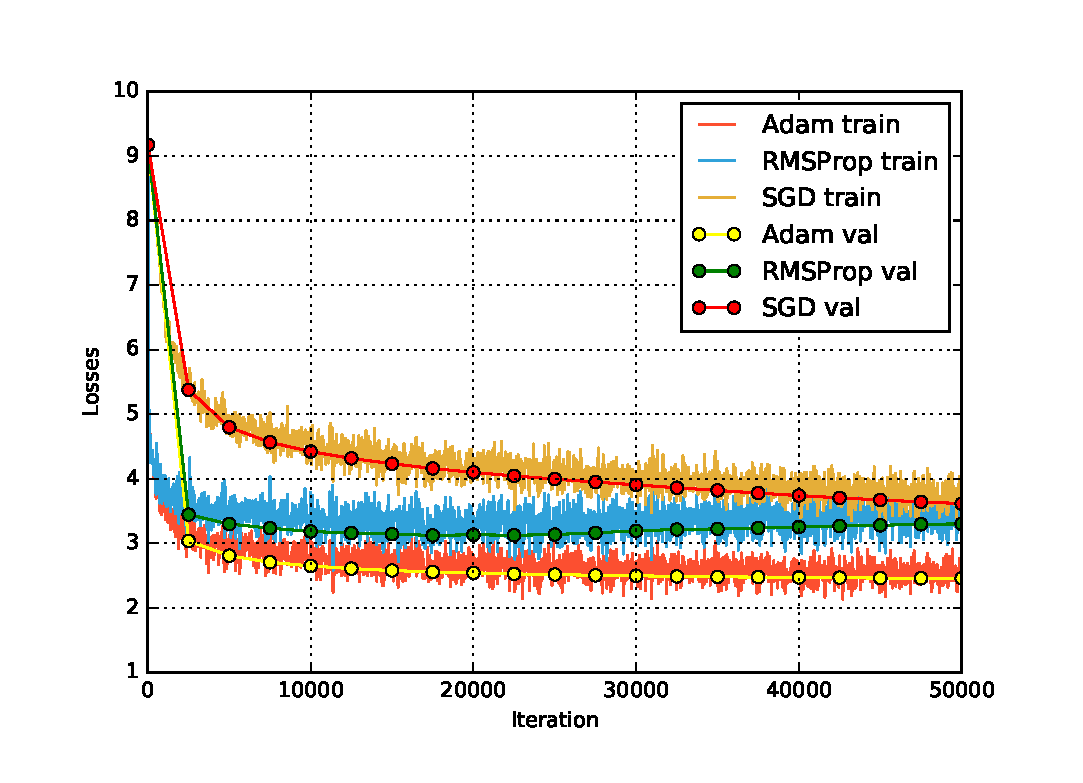
\includegraphics[width=0.48\linewidth]{Chapters/Fig/vgg_optims.eps}
			\hfill
			\includegraphics[width=0.48\linewidth]{Chapters/Fig/vgg_lang_stat.eps}
		}
		\subfigure[Config-2: AlexNet as CNN, LSTM with $512$ hidden units]{
			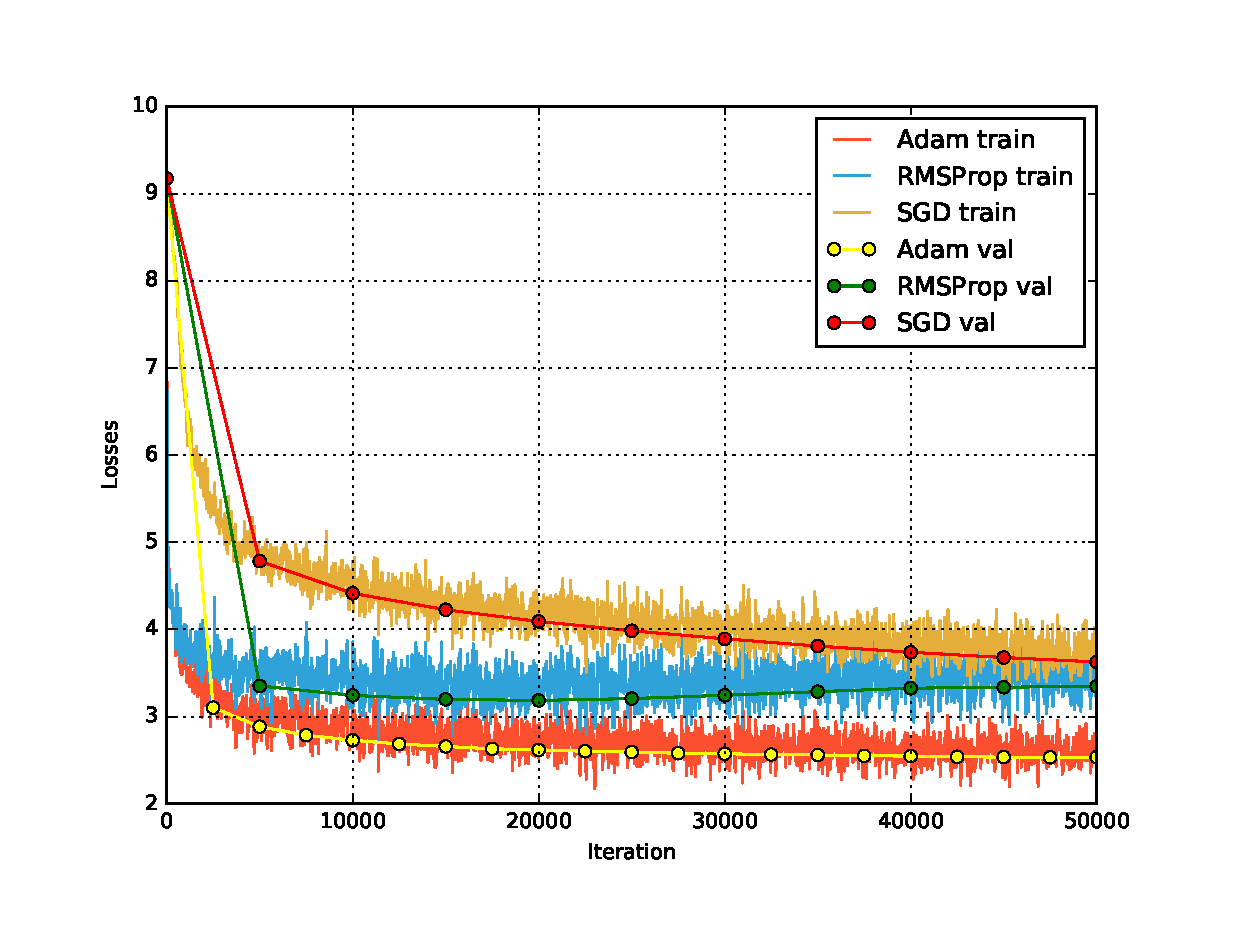
\includegraphics[width=0.48\linewidth]{Chapters/Fig/alex_optims.eps}
			\hfill
			\includegraphics[width=0.48\linewidth]{Chapters/Fig/alex_lang_stat.eps}
		}
		\caption[Comparison of $3$ opitmization methods ]{Comparison of $3$ optimization methods: SGD, RMSProp and Adam w.r.t training/validation losses and language evaluation score during the first $50,000$ training iterations}
		\label{fig:exp1} % label should be placed immediately after \caption for cross-reference to work properly
	\end{figure}

The train and validation losses as well as language evaluation scores during the first $50,000$ iterations for each configuration are shown in Figure \ref{fig:exp1}. 

As can be inferred from figure \ref{fig:exp1}, regardless of the \gls{cnn}, Adam optimizer gives the fastest convergence rate; pure \gls{sgd} without momentum and weight decay gives the lowest convergence rate compared the other optimization methods. In addition, the losses reach a ``plateau'' (approximately $2.5$) very quickly after about first $20,000$ iterations, which indicates that the chose learning rate is considerably good enough for this problem.  

Regarding the language evaluation scores on standard metrics, both Adam and RMSProp achieves superior results to SGD, with Adam performs slightly better. The BLEU-1 and METEOR scores for SGD is fluctuated, which reflects its lower convergence rate compared to Adam and RMSProp.

Following the monitoring stragies presented in section \ref{sec:monitoring}, we kept training and monitoring the behavoirs of the models with different settings. The training was terminated if the gradient is exploded (which did not happen for all experiments shown in this thesis) or when the CIDEr score was not improved after $50,000$ consecutive iterations to prevent overfitting. 

On hardware environment mentioned in section \ref{sec:hardware}:
\begin{itemize}
	\item Config-1
	\begin{itemize}
		\item \textit{Adam optimizer}: takes approximately $20$ hours to train and achieves the best results at iteration $94,000$-th. 
		\item \textit{RMSProp optimizer}: training time is $29,4$ hours and achieves the best results at iteration $138,000$-th.
		\item \textit{SGD optimizer}: training finished after $38,2$ hours and achieves the best results at iteration $272,000$-th
	\end{itemize}
	\item Config-2
	\begin{itemize}
		\item \textit{Adam optimizer}: takes approximately $23$ hours to train and achieves the best results at iteration $146,500$-th. 
		\item \textit{RMSProp optimizer}: training time is $30,3$ hours and achieves the best results at iteration $191,000$-th.
		\item \textit{SGD optimizer}: training finished after $42,5$ hours and achienves the best results at iteration $189,000$-th
	\end{itemize}
\end{hardware}

The BLEU, METEOR and CIDEr scores for this experiment are reported in Table \ref{tab:exp1_coco_score}

\renewcommand{\arraystretch}{1.2}

\begin{table}
	\centering
	\begin{tabular}{llcccccc}
		\toprule
		Configuration & Optimizer & B-1 & B-2 & B-3 & B-4 & METEOR & CIDEr \\ \midrule
		\multirow{3}{*}{\textit{Config-1}} & Adam & \textbf{62.9} & & & & 21.2 & \textbf{65.5} \\
		 & RMSProp & 61.8 & & & & 19.7 & 62.4 \\
		 & SGD & 55.5 & & & & 15.5 & 32.3 \\
		 \midrule
		 \multirow{3}{*}{\textit{Config-2}} & Adam & 61.5 & & & &\textbf{21.5} & 63.7 \\
		 & RMSProp & 60.2 & & & & 18.9 & 61.2 \\
		 & SGD & 53.1 & & & & 14.0 & 30.8 \\
		 \midrule
		 LRCN\cite{DBLP:journals/corr/DonahueHGRVSD14} &  & 62.8 & 44.2 & 30.4 & -- & -- & -- \\
		 BRNN\cite{DBLP:journals/corr/KarpathyF14} & & 62.5 & 45.0 & 32.1 & 23.0 & 19.5 & 66.0 \\
		 Google NIC \cite{DBLP:journals/corr/VinyalsTBE14} & & 66.6 & 46.1 & 32.9 & 24.6 & -- & -- \\
		 Nearest Neighbor \cite{DBLP:journals/corr/KarpathyF14} & & 48.0 & 28.1 & 16.6 & 10.0 & 15.7 & 38.3 \\ 
		 \bottomrule
	\end{tabular}
	\caption[Evaluation of image captions generated on $1000$ test images]{Evaluation of image captions generated on 1000 test images. \textbf{B-n} is BLEU score that uses up to n-grams. High is good in all columns. }
	\label{tab:exp1_coco_score}
\end{table}

\textbf{Conclusion:} With both VGGNet and AlexNet as the CNN module of the model, Adam $( \eta = 5\mathrm{e}{-4}$; $\alpha = 0.8, \beta = 0.999, \epsilon = 1\mathrm{e}{-8} )$ gives the best results in terms of the model convergence rate. Therefore, it will be used as the optimization method in the subsequent experiments.

% -------------------------------------------------------------------
%    				Exp 2: LSTM Architecture
% -------------------------------------------------------------------
\subsection{Experiment 2: LSTM Architecture}
\label{exp:lstm_architecture}
\subsubsection{Experimental setup}
As studied in \cite{DBLP:journals/corr/GreffSKSS15}, beside the learning rate $\eta$, the hidden layer size $h$ is an important hyperparameter that affects the performance of \gls{lstm} network. 
This experiment is conducted to evaluate the effects of different hidden sizes $h$ to the captioning model so as to figure out a suitable one as a trade-off between the performance of the model and the required training time as well as the computational capability of machine used in inference phase.
To this end, I consider three different values of $h$ that are largely used in researches of \gls{lstm}. %, specifically $h = \left\{ 256, 512, 1000\right\}$. 
The learning rate is set to $\eta = 5\mathrm{e}{-4}$, and the optimization method is Adam.

\subsubsection{Experimental results and evaluations}
\begin{figure}[ht]
	\subfigure[VGGNet as CNN; Adam optimizer]{
		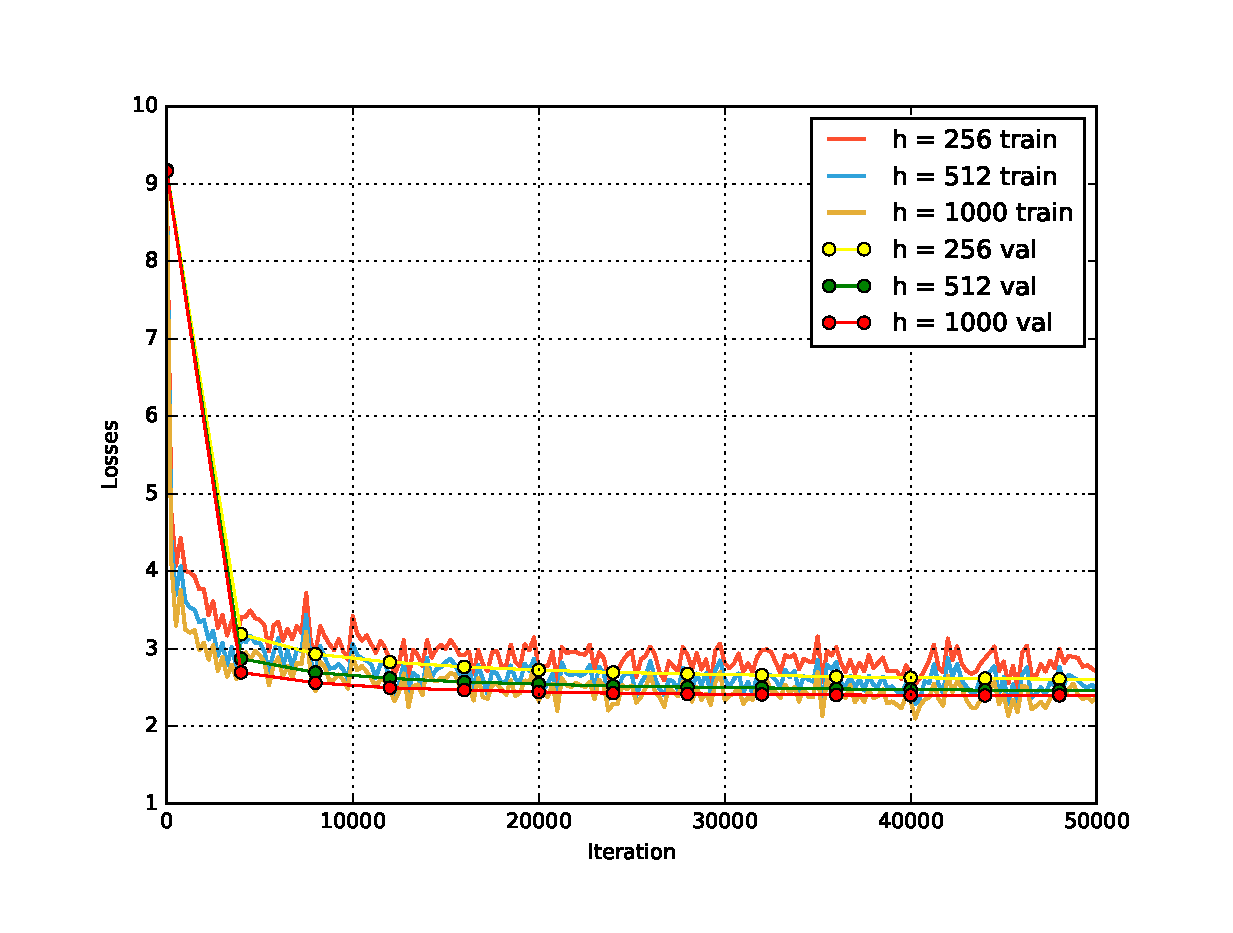
\includegraphics[width=0.48\linewidth]{Chapters/Fig/vgg_hiddens.eps}
		\hfill
		\includegraphics[width=0.48\linewidth]{Chapters/Fig/vgg_hidden_lang_stat.eps}
	}
	\subfigure[AlexNet as CNN; Adam optimizer]{
		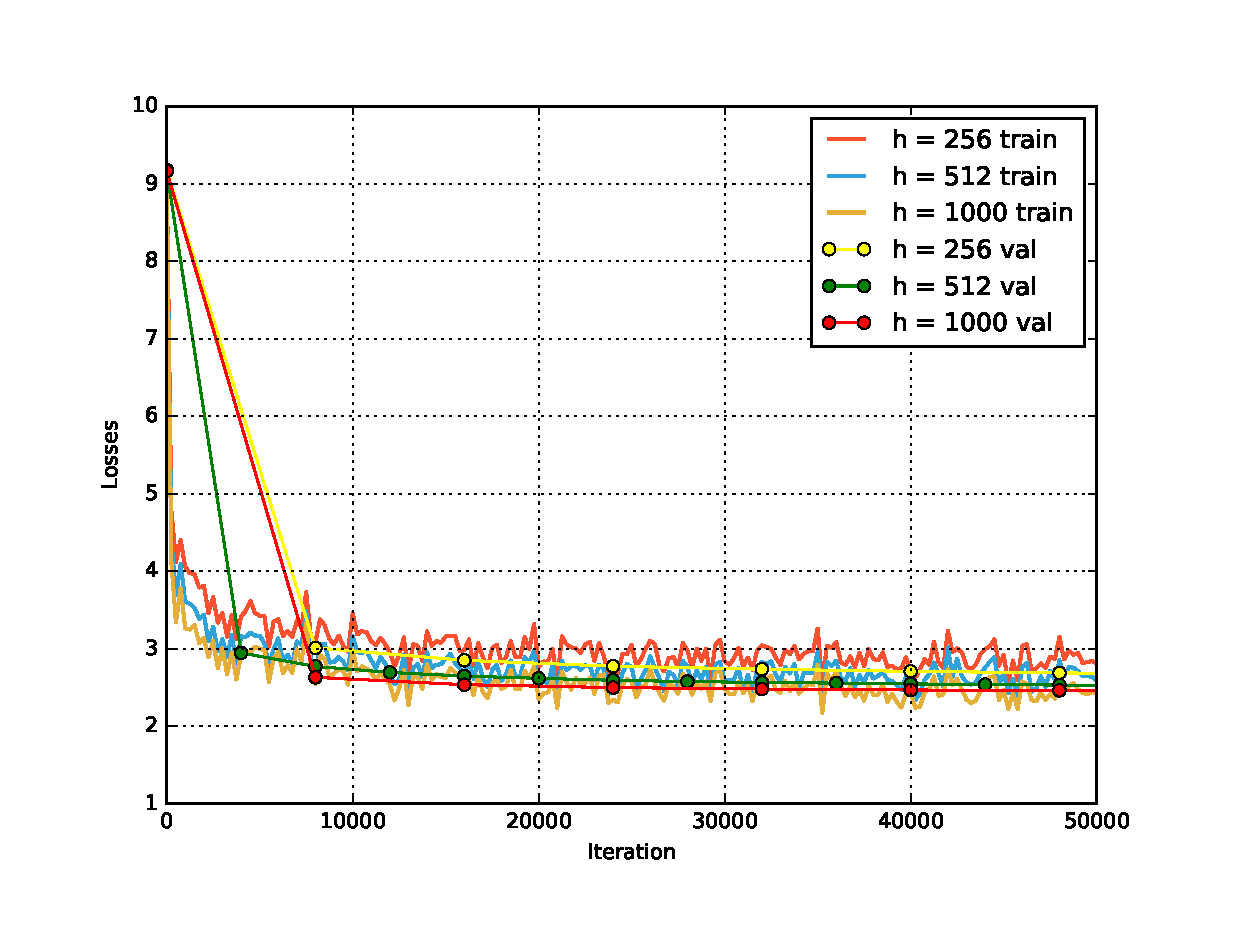
\includegraphics[width=0.48\linewidth]{Chapters/Fig/alex_hiddens.eps}
		\hfill
		\includegraphics[width=0.48\linewidth]{Chapters/Fig/alex_hidden_lang_stat.eps}
	}
	\caption[Comparison of $3$ LSTM hidden sizes]{Comparison of $3$ LSTM hidden sizes: $h \in \left\{ 256, 512, 1000 \right\}$ w.r.t training/validation losses and language evaluation score during the first $50,000$ training iterations}
	\label{fig:exp2} % label should be placed immediately after \caption for cross-reference to work properly
\end{figure}

The plots in Figure \ref{fig:exp2} show that all three LSTM hidden sizes result in the remarkably similar convergence rates, both training and validation losses converges quickly. Furthermore, as expected, larger networks perform better,
however the required training time and the number of network's parameters are also considerably increased. As a result, the model might not be usable when it is deployed to different machines at the inference time even though inference is just forwarding the inputs to the model.

% // \textit{TODO: Perform experiments on different LSTM architecture }
% Another unexpected result of this experiment is that momentum affects neither performance nor training time in any significant way. ...
% These observations suggest that momentum does not offer substaintial benefits when training LSTMs with online stochastic gradient descent as it does with the case of \gls{cnn}. It may, however, be more important in the case of batch training in which the gradient is less noisy.

\textbf{Conclusion:} In the context of this experiment, the differences of convergence rate and performance of the model are not significant amongst three hidden size values evaluated. Nonetheless, as predefined above, the ultimate goal of this experiment is not to point out the best model in some certain extents but to figure out the trade-offs between model's performance versus the feasibility of deploying that model to wide varieties of hardware infrastructure. To this end, the good choice is an LSTM with $h = 512$ and \texttt{tanh} nonlinearity for its forget gate.

% -------------------------------------------------------------------
%    				Exp 3: AlexNet and VGGNet
% -------------------------------------------------------------------
\subsection{Experiment 3: AlexNet vs VGGNet}
\label{exp:cnn}
As mentioned in previous chapter, the very first stage of our model is to feed input image into a convolutional neural network to extract a fixed-length representation (feature vector) of that image. This vector together with the embedded vector of groundtruth sentence are then used as inputs to the LSTM decoder. Thus, a good CNN, which can extract salient information from the raw image, is essentially an important component of our captioning model. Recent advanced computer vision system often utilize very deep CNNs \footnote{VGGNet has 16 layers, GoogLeNet has 32 layers and the Residial Network - ResNet has up to 152 layers} with the argument that deeper networks work better. Nonetheless, deeper network comes with much larger number of parameters and is computationally expensive (even only for a single forward pass through the network). 

\subsubsection{Experimental setup}
With the goal to find a reasonable trade-off between performance and portability of the model, we comparatively evaluate the AlexNet \cite{NIPS2012_4824} and VGGNet \cite{Simonyan14c} as the vision part of our models. To this end, we fix other settings as follow: Adam ($\alpha = 0.01, \beta_1 = 0.99, \beta_2 = 0.999, \epsilon = 10^{-8}$), the LSTM has $h = 512$ hidden units.

\subsubsection{Experimental results and evaluation}

	\begin{table}
		\centering
		\caption{Comparision between AlexNet and VGGNet as the vision module of captioning models}
		\label{tab:cnn_compare}

		\begin{tabular}{l{2cm}cc}
			\toprule
				& \textbf{AlexNet} & \textbf{VGGNet-16} \\
			\midrule
			\#parameters of the CNN & $56,723,488$ & $136,358,208$\\
			\#parameters of captioning model & $68,631,936$ & $148,266,656$ \\
			Size of model & $207$ MB & $566$ MB\\
			\midrule
			Time for single forward on GPU & & \\
			Time for single forward on CPU & & \\
			\bottomrule
		\end{tabular}
	\end{table}

Table \ref{tab:cnn_compare} shows the details of our models with different CNNs. It is easy to see that the CNN constitues a large portion of parameters to captioning models and the number of parameters with AlexNet as CNN is only half of those with 16-layer VGGNet as CNN, so is the size of captioning models.

\begin{figure}
	\centering
	\includegraphics[width=\linewidth]{Chapters/Fig/vgg_prediction_on_coco.pdf}
	\caption{A random selection of generated captions by the model with VGGNet as its vision module}
	\label{fig:vgg_captions}
\end{figure}

Figure \ref{fig:vgg_captions} shows some randomly selected captions generated by our models with VGGNet as its vision component. We manually evaluate and classify the captions into four groups:

\begin{itemize}
	\item \textit{Describe without errors:} the generated caption can precisely describe the content of the image. The details of objects, colors, positions, actions, etc. might not necessarily included in the caption. Nevertheless, once those details are mentioned in the caption, their description needs to be correct.
	\item \textit{Describe with minor errors:} there can be minor errors regarding the number, the color, etc. of objects described in the description
	\item \textit{Somewhat related to the image:} the caption can describe correctly some portions of the image
	\item \textit{Unrelated to the image:} the caption cannot describe visual contents of the image and has completely different semantic meaning to what is in the image, which can lead to the misunderstanding about the content of the image.
\end{itemize}

As can be seen from Figure \ref{fig:vgg_captions}, our models generate sensible captions that describe various kind of image fairly well. Even though there is no explicit information of the grammar of groundtruth sentences in the training set, the genrated sentences are ensured in grammar correctness. In addition, the captions are able to reflect salient information of the image; notice that in the second image of the first column, the models can capture the ``bat'' given its size and the fact that we do not incorporate any object detection machenism in our models.

%-------------------------------------------------------------------
%    				Exp 4: Transfer learning
% -------------------------------------------------------------------
\subsection{Experiment 4: Transfer learning}
\label{exp:transfer_learning}

Transfer learning is the process of transfering the learnt representation (knowledge) from related \textit{source} to \textit{target} domains \cite{Pan:2010:STL:1850483.1850545}. Deep networks often contain millions of parameters and are trained on large datasets. The training process can be cumbersome and require carefully chosen weight initialization strategies, optimization methods and most prominently a lot of time. Therefore, one can utilise transfer learning to boost up the training. 

The usual transfer learning approach is to first train a base network on a base dataset, and then repurpose its first $n$ layers to the first $n$ layers of the target network \cite{DBLP:journals/corr/YosinskiCBL14}. The remaing layers of target network are randomly initialized and trained on the target dataset w.r.t to the target dataset.

\subsubsection{Experimental Setup}

In this experiment, all the layers from model trained in MSCOCO dataset are transferred to learn in new Flickr 30k dataset. The CNN module is VGGNet-16, the learning rate $\eta = 5\mathrm{e}{-4}$, the optimizer is Adam with $\alpha = 0.8, \beta = 0.999, \epsilon = 1\math{e}{-8}$. The LSTM has $512$ hidden units. The performance of the model is reported by BLEU metric (in Table \ref{tab:exp4_flickr_score}).

\begin{table}
	\centering
	\caption{Scores on Flickr30k 1000 test images in transfer learning}
	\label{tab:exp4_flickr_score}
	\begin{tabular}{lcccc}
		\toprule
		Optimizer & BLEU-1 & BLEU-2 & BLEU-3 & BLEU-4 \\ \midrule
		SGD & 50.4 & 31.4 & 19.0 & 12.4 \\
		RMSProp & 52.9 & 33.1 & 20.1 & 12.8 \\
		Adam & 53.9 & 34.4 & 21.3 & 13.7 \\
		\midrule
		LRCN\cite{DBLP:journals/corr/DonahueHGRVSD14} & 58.8 & 39.1 & 25.1 & 16.5  \\
		BRNN\cite{DBLP:journals/corr/KarpathyF14} & 57.3 & 36.9 & 24.0 & 15.7  \\
		Google NIC \cite{DBLP:journals/corr/VinyalsTBE14} & 66.3 & 42.3 & 27.7 & 18.3 \\
		\bottomrule
	\end{tabular}
\end{table}

\subsubsection{Experimental results and evaluations}

\begin{figure}[ht]
	\centering
	\subfigure[Training/validation losses for first $50,000$ iteration]{
		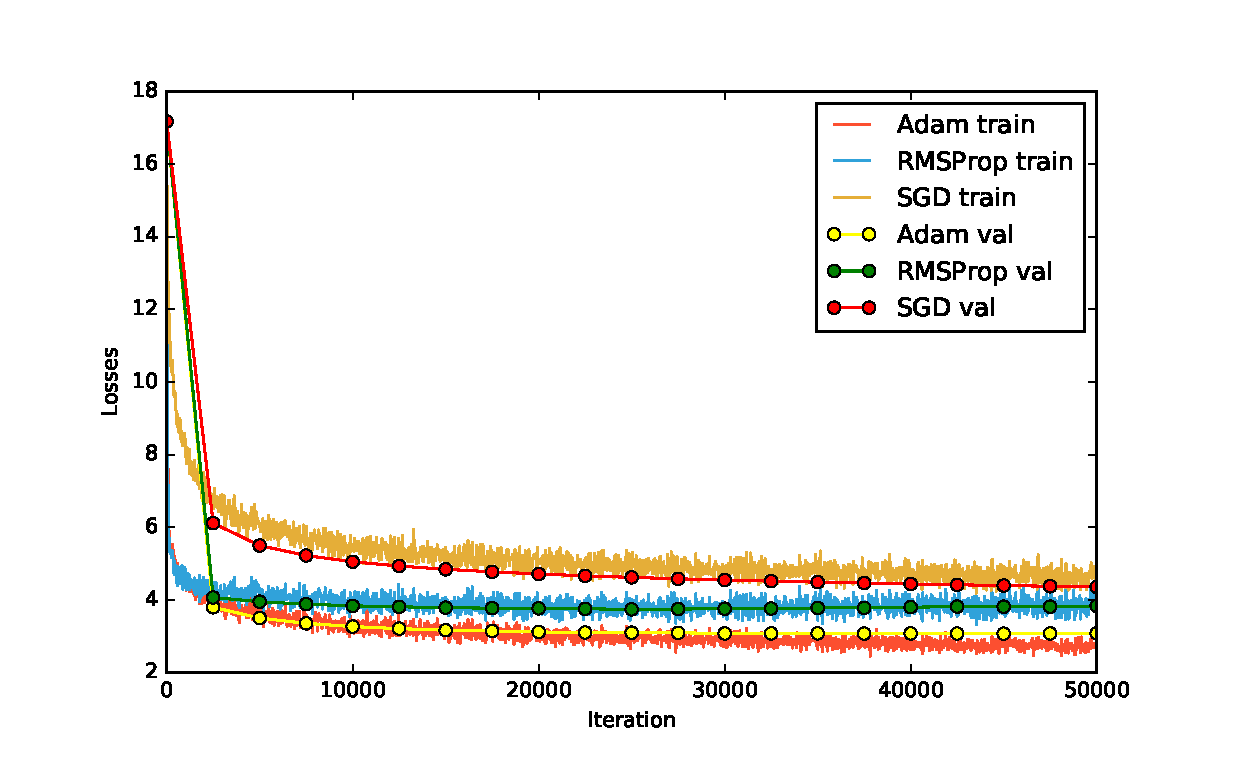
\includegraphics[width=0.8\textwidth]{Chapters/Fig/transfer_flickr30k_train_val.eps}
		\hfill
	}
	\subfigure[BLEU scores on Flickr30k dataset]{
		\includegraphics[width=0.8\textwidth]{Chapters/Fig/transfer_flickr30k_langeval.eps}
		\hfill
	}
	\caption{Transfer learning on Flickr30k dataset}
	\label{fig:exp_4} % label should be placed immediately after \caption for cross-reference to work properly
\end{figure}

As can be inferred from Figure \ref{fig:exp_4}(a), the convergence on this experiment are similar to those in the previous experiments. Specifically, the objective function converges quickly within the first $10,000$ iterations and Adam still gives the best convergence scheme. 

According to Table \ref{tab:exp4_flickr_score}, all the scores are degraded by approximately $10$ points. This degration can be explained by the dissimilarity between MSCOCO and Flickr 30k datasets as indicated in \cite{DBLP:journals/corr/YosinskiCBL14}. Even though MSOCO is 5 times bigger than Flickr 30k, the collection of those two datasets was done differently, which results in vocabulary differences and larger mismatch. In addition, an interesting finding is that despite the ``smooth'' shapes of training/validation losses, the BLEU score evolution showcases a different characteristics. Concretely, with SGD, the BLEU score fluctuates with large variance (for BLEU-1) compared to the relatively ``smooth'' shape of BLEU score of Adam and RMSProp. Nevertheless, the general trend is that BLEU score in all cases are quickly boosted up after first $5,000$ iterations which confronts with the learning curves in Figure \ref{fig:exp_4}a.

Next, I visually examine sample generated captions by this transfer learning. 

// TODO: run \texttt{eval.lua} to produce captions for Flickr30k test images and sample 16 images, classify them into 4 groups: describe without errors, describe with minor errors, somewhat related to the image, unrelated to the image.